\documentclass[xcolor=table,final]{beamer} %,handout
\usepackage{etex}

\usepackage{amsfonts,amssymb}
\usepackage{url}
\usepackage{physics}
%% \usepackage{hyperref}

\usepackage[T2A]{fontenc}
\usepackage[utf8]{inputenc}
\usepackage[english]{babel}
\usepackage[linesnumbered,vlined]{algorithm2e}
\usepackage{booktabs}
\usepackage{fancybox}
\usepackage{blockmatrgraph}

\usepackage{tikz}
\usetikzlibrary{matrix,shadows,arrows,shapes,patterns,trees}
\usepackage{dirtree}

\usepackage{ulem}
\usepackage{bbm}

\newcommand{\PageRank}{\texttt{PageRank}\xspace}
\newcommand{\TrustRank}{\texttt{TrustRank}\xspace}
\newcommand{\MapReduce}{\texttt{MapReduce}\xspace}
\newcommand{\ones}{\mathbbm{1}}

\newcommand{\Bsof}{\texttt{BSOF}\xspace}
\newcommand{\Bstri}{\texttt{BSTRI}\xspace}
\newcommand{\Bsoftri}{\texttt{BSOFTRI}\xspace}
\newcommand{\Bsoi}{\texttt{BSOI}\xspace}
\newcommand{\Gemm}{\texttt{DGEMM}\xspace}
\newcommand{\Trmm}{\texttt{DTRMM}\xspace}
\newcommand{\Trsm}{\texttt{DTRSM}\xspace}
\newcommand{\Lacpy}{\texttt{DLACPY}\xspace}
\newcommand{\Trtri}{\texttt{DTRTRI}\xspace}
\newcommand{\Geqrf}{\texttt{DGEQRF}\xspace}
\newcommand{\Orgqr}{\texttt{DORGQR}\xspace}
\newcommand{\Ormqr}{\texttt{DORMQR}\xspace}
\newcommand{\Ilaenv}{\texttt{ILAENV}\xspace}

\mode<presentation>{
  \hypersetup{pdfpagemode=FullScreen}
  
  %% \usetheme{Berkeley}
  %% \usecolortheme{crane}%{seagull}
  %% \usetheme{AnnArbor}
  \usecolortheme{rose}

  \setbeamercovered{transparent}
}

\mode<handout>{
  \useinnertheme{default}
  \useoutertheme{infolines}
  \usecolortheme{default}
  \usefonttheme{professionalfonts}

  \usepackage{pgfpages}
  \pgfpagesuselayout{2 on 1}[a4paper,border shrink=4mm]

  \setbeamercolor{structure}{fg=black}
  \setbeamerfont{structure}{series=\bfseries} 
}

\title[PageRank and Kempe-McSherry]{%
  Applying Orthogonal/Power Iterations to Big Graph Mining : \PageRank and Kempe-McSherry Algorithms}
\subject{Big Graph Mining}

\author[S.\,Gogolenko]{
  Sergiy Gogolenko %\inst{1} 
}

\institute[DonNTU]{%
  
\includegraphics[height=2cm]{./figs/logo/donntu-logo.png}%Donetsk National Technical University
  \hspace*{0.75cm}~%
  
\includegraphics[height=2cm]{./figs/logo/ucu-logo.png}%University of California, Davis
}
%% \titlegraphic{
\includegraphics[width=4cm]{./figs/logo/ucdavis-logo.png}}

\date[Lviv 2016] {%
  Ukrainian Catholic University, Lviv \\%
  \footnotesize{2016, May 23}
}


\pgfdeclareimage[height=1.2cm]{university-logo}{./figs/logo/ucdavis-logo.png}

\begin{document}

\frame[plain]{\titlepage}

\begin{frame}{Outline}%[pausesections]{Outline}
  \tableofcontents
\end{frame}

\section{\PageRank}

% %% \subsection{Problem formulation}

% \begin{frame}{Problem formulation}
%   \begin{definition}[$p$-cyclic matrix]
%     \begin{equation} \label{eq:matr_A}
%       H =
%       \begin{bmatrix}
%         A_1 &    &    &  & B_p   \\
%         B_1 & A_2 &    &  &  \\
%         & B_2 & A_3 &  &     \\
%         &        & \ddots & \ddots &         \\
%         &     &          & B_{p-1} & A_p
%       \end{bmatrix}
%       ,
%     \end{equation}
%     where $A_i$ and $B_i$ are non-zero blocks
%   \end{definition}
% \end{frame}

%%%%%%%%%%%%%%%%%%%%%%%%%%%%%%%%%%%%%%%%


\begin{frame}{\PageRank}%{What made them heros of top magazine cover?}
  \begin{columns}
    \column[T]{0.5\textwidth}
\begin{center}
    Sergey Brin

    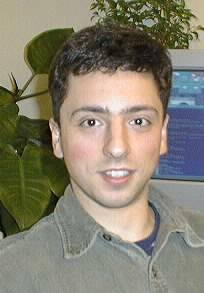
\includegraphics[width=0.7\textwidth]{figs/extras/sergey-brin}
\end{center}
    
    \column[T]{0.5\textwidth}
\begin{center}
    Larry Page

    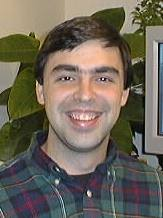
\includegraphics[width=0.7\textwidth]{figs/extras/larry-page}

\end{center}
  \end{columns}

  \begin{center}
    % http://infolab.stanford.edu/~backrub/google.html
    \textit{The Anatomy of a Large-Scale Hypertextual Web Search Engine} \\
    Computer Science Department, Stanford University \\
    1998
  \end{center}
% Sergey Brin and Lawrence Page
% {sergey, page}@cs.stanford.edu
% 
\end{frame}
%%%%%%%%%%%%%%%%%%%%%%%%%%%%%%%%%%%%%%%%
\begin{frame}{\PageRank}{What made them heros of top magazine cover?}
  \begin{columns}
    \column[T]{0.5\textwidth}
    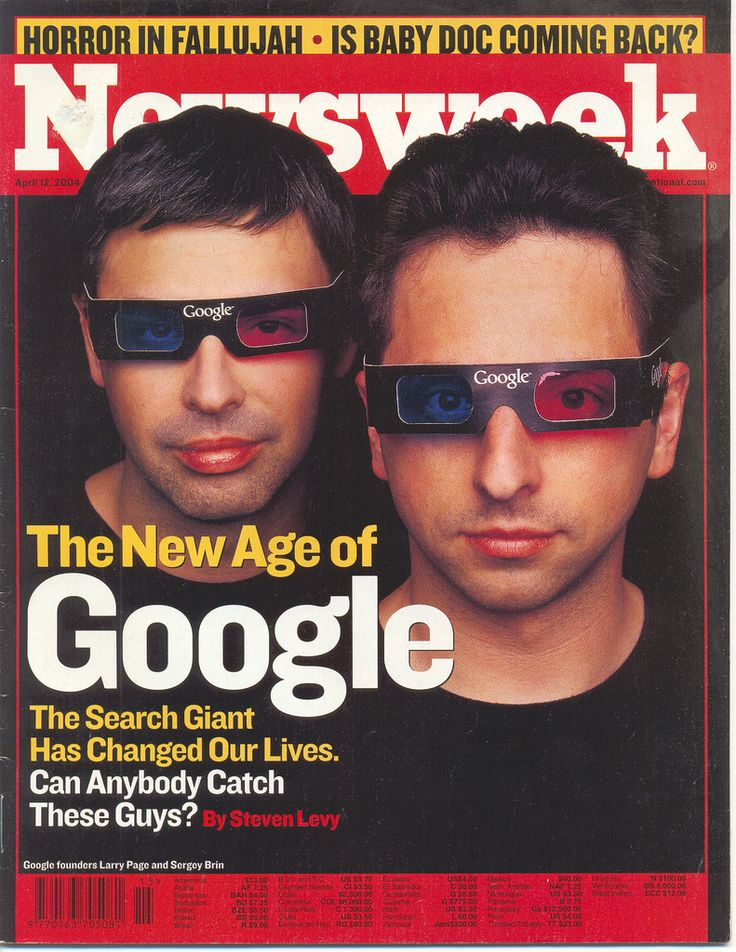
\includegraphics[width=1.\textwidth]{figs/extras/brin-page-newsweek1}

    .
    \column[T]{0.5\textwidth}
    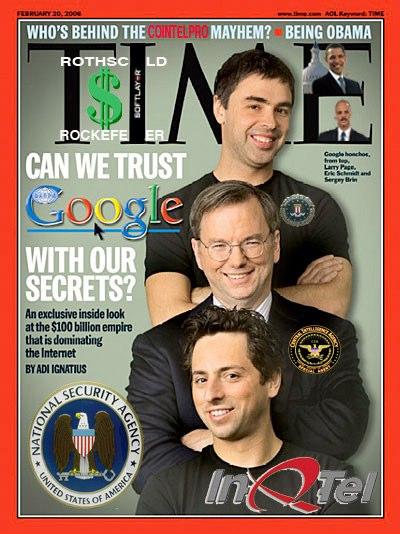
\includegraphics[width=1.\textwidth]{figs/extras/brin-page-time}
  \end{columns}
\end{frame}
%%%%%%%%%%%%%%%%%%%%%%%%%%%%%%%%%%%%%%%%
\subsection{Model and basic algorithm}
%%%%%%%%%%%%%%%%%%%%%%%%%%%%%%%%%%%%%%%%
\begin{frame}{\PageRank : The model}{Measure of importance}
  \begin{columns}
    \begin{column}{0.3\textwidth}
      
\includegraphics[width=1.\textwidth]{figs/extras/penguin-no-spam}%{figs/extras/google-webspam}
    \end{column}
    \begin{column}{0.7\textwidth}

      % \structure{SP}iced h\structure{AM}

      \begin{exampleblock}{}%{Key}
        % While Google was not the first search engine, 
        % it was the first able to defeat the spammers who had made search almost useless.

        The \structure{importance} of a Web page is an inherently subjective matter...%, which depends on the readers interests, knowledge and attitudes. 
        But there is still much that can be said \alert{objectively} about the \structure{relative importance} of Web pages.

        \href{http://ilpubs.stanford.edu:8090/422/}{{\tiny
            \underline{Page, L.}; \underline{Brin, S.}; Motwani, R.; Winograd, T. (\underline{1999}) 
            \textit{The \textbf{PageRank} Citation Ranking: Bringing Order to the Web}. Tech.rep. \underline{Stanford} InfoLab.}}
      \end{exampleblock}
    \end{column}
  \end{columns}
  \pause
  \begin{centering}
    \structure{\fbox{Probability of visiting page by idealized random Web surfer}}
  \end{centering}
  \begin{block}{Why this trick works?}
    \begin{itemize}
    \item users of the Web ``vote with their feet'' %tend to place links to pages they think are good or useful
    \item users are more likely to visit useful pages
    \end{itemize}
  \end{block}
\end{frame}
%%%%%%%%%%%%%%%%%%%%%%%%%%%%%%%%%%%%%%%%
\begin{frame}{\PageRank : The model}{Random surfing as Markov process}
  % probability distribution for the location of a random surfer
  \begin{columns}
    \column{0.2\textwidth}
    
\includegraphics[width=1.\textwidth]{figs/extras/web-surfer}
    \column{0.45\textwidth}
    \includegraphics<1>[width=1.\textwidth]{figs/tex/graph}
    \includegraphics<2>[width=1.\textwidth]{figs/tex/graph_probability0}
    \includegraphics<3>[width=1.\textwidth]{figs/tex/graph_probability1}
    \includegraphics<4>[width=1.\textwidth]{figs/tex/graph_probability2}
    \column{0.4\textwidth}
    
    \begin{exampleblock}{Probabilities}
      \begin{enumerate}
      \item<2-> $\Pr = (1,0,0,0,0)$
      \item<3-> $\Pr = (0,0,0,0,1)$
      \item<4-> $\Pr = (0,\frac{2}{5},\frac{2}{5},\frac{1}{5},0)$
      \end{enumerate}
    \end{exampleblock}
  \end{columns}

  \pause 
  \begin{block}{Probability evolution}
    \structure{
      \begin{equation*}
        {\Pr}'(x) = \sum_{y \to x} \frac{\Pr(y)}{\deg^+(y)}
      \end{equation*}
    }
    {\small
      \begin{itemize}
      \item $\deg^+(y)$ -- outdegree of $y$
      \end{itemize}
    }
  \end{block}
\end{frame}
%%%%%%%%%%%%%%%%%%%%%%%%%%%%%%%%%%%%%%%%
\begin{frame}{\PageRank : The model}{Transition matrix of the Web}
  % probability distribution for the location of a random surfer

  \begin{columns}
    \column{0.45\textwidth}
    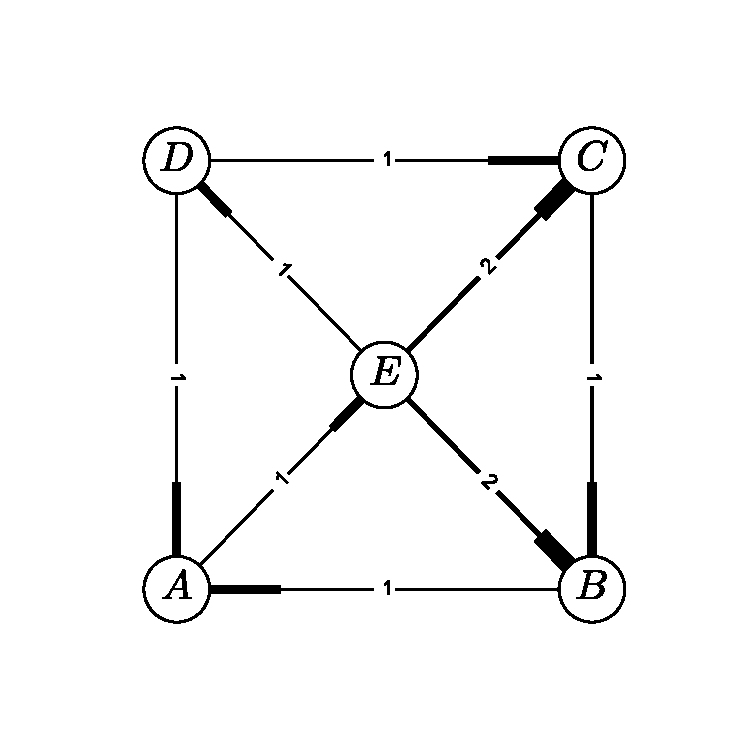
\includegraphics[width=1.\textwidth]{figs/tex/graph}
    %\begin{exampleblock}<1>{Matrix-vector representation}
      \structure{
        \begin{equation*}
          M =
          \left[\begin{matrix}0 & 1 & 0 & \frac{1}{2} & 0\\0 & 0 & 1 & 0 & \frac{2}{5}\\0 & 0 & 0 & \frac{1}{2} & \frac{2}{5}\\0 & 0 & 0 & 0 & \frac{1}{5}\\1 & 0 & 0 & 0 & 0\end{matrix}\right]
        \end{equation*}
      }
      % \end{exampleblock}

    \column{0.55\textwidth}
   \begin{block}{Matrix-vector representation}
     \structure{
       \begin{equation*}
         {\Pr}' = M \cdot {\Pr}
       \end{equation*}
     }
     \begin{itemize}
     \item $M$: 
       $m_{xy}=\begin{cases}1/\deg^+(y), & y \to x\\ 0, &y \not\to x \end{cases}$
     \end{itemize}
     % A matrix whose column sums are at most 1 is called \structure{substochastic}
     $M$ is \structure{stochastic} matrix
     \begin{equation*}
       \forall y: \sum_x m_{xy} = 1
     \end{equation*}
   \end{block}
  \end{columns}

\end{frame}
%%%%%%%%%%%%%%%%%%%%%%%%%%%%%%%%%%%%%%%%
\begin{frame}{\PageRank : The model}{Simulation of random surfer}
  \begin{columns}
    \column[T]{0.45\textwidth}
    \includegraphics<1>[width=1.\textwidth]{figs/tex/graph_tansmatr0}
    \includegraphics<2>[width=1.\textwidth]{figs/tex/graph_tansmatr1}
    \includegraphics<3>[width=1.\textwidth]{figs/tex/graph_tansmatr2}
    \includegraphics<4>[width=1.\textwidth]{figs/tex/graph_tansmatr3}
    \includegraphics<5->[width=1.\textwidth]{figs/tex/graph_tansmatrN}

    \column[T]{0.55\textwidth}
    \begin{exampleblock}{Simulation of random surfer}
      \only<1>{
        { ${\Pr}^i$ probability distribution for the location of a random surfer at step $i$}
          \begin{align}
            {\Pr}^0 &= \left[\begin{matrix}\frac{1}{5}&\frac{1}{5}&\frac{1}{5}&\frac{1}{5}&\frac{1}{5}\end{matrix}\right]^T \\
            {\Pr}^{i+1} &= M \cdot \Pr^{i}
          \end{align} 
        }
      \only<2>{ \begin{equation*}
          \left[\begin{matrix}\frac{3}{10}\\\frac{7}{25}\\\frac{9}{50}\\\frac{1}{25}\\\frac{1}{5}\end{matrix}\right] = 
          \left[\begin{matrix}0 & 1 & 0 & \frac{1}{2} & 0\\0 & 0 & 1 & 0 & \frac{2}{5}\\0 & 0 & 0 & \frac{1}{2} & \frac{2}{5}\\0 & 0 & 0 & 0 & \frac{1}{5}\\1 & 0 & 0 & 0 & 0\end{matrix}\right]
          \times
          \left[\begin{matrix}\frac{1}{5}\\\frac{1}{5}\\\frac{1}{5}\\\frac{1}{5}\\\frac{1}{5}\end{matrix}\right]
        \end{equation*} }

      \only<3>{ \begin{equation*}
          \left[\begin{matrix}\frac{3}{10}\\\frac{13}{50}\\\frac{1}{10}\\\frac{1}{25}\\\frac{3}{10}\end{matrix}\right] = 
          \left[\begin{matrix}0 & 1 & 0 & \frac{1}{2} & 0\\0 & 0 & 1 & 0 & \frac{2}{5}\\0 & 0 & 0 & \frac{1}{2} & \frac{2}{5}\\0 & 0 & 0 & 0 & \frac{1}{5}\\1 & 0 & 0 & 0 & 0\end{matrix}\right]
          \times
          \left[\begin{matrix}\frac{3}{10}\\\frac{7}{25}\\\frac{9}{50}\\\frac{1}{25}\\\frac{1}{5}\end{matrix}\right]
        \end{equation*} }

      \only<4>{ \begin{equation*}
          \left[\begin{matrix}\frac{7}{25}\\\frac{11}{50}\\\frac{7}{50}\\\frac{3}{50}\\\frac{3}{10}\end{matrix}\right] = 
          \left[\begin{matrix}0 & 1 & 0 & \frac{1}{2} & 0\\0 & 0 & 1 & 0 & \frac{2}{5}\\0 & 0 & 0 & \frac{1}{2} & \frac{2}{5}\\0 & 0 & 0 & 0 & \frac{1}{5}\\1 & 0 & 0 & 0 & 0\end{matrix}\right]
          \times
          \left[\begin{matrix}\frac{3}{10}\\\frac{13}{50}\\\frac{1}{10}\\\frac{1}{25}\\\frac{3}{10}\end{matrix}\right]
        \end{equation*} }

      \only<5>{\small \begin{equation*}
          \underbrace{\left[\begin{matrix}0.28\\0.25\\0.14\\0.06\\0.28\end{matrix}\right]}_{{\Pr}^{\infty}} = 
          \underbrace{\left[\begin{matrix}0 & 1 & 0 & \frac{1}{2} & 0\\0 & 0 & 1 & 0 & \frac{2}{5}\\0 & 0 & 0 & \frac{1}{2} & \frac{2}{5}\\0 & 0 & 0 & 0 & \frac{1}{5}\\1 & 0 & 0 & 0 & 0\end{matrix}\right]}_{M}
          \times
          \underbrace{\left[\begin{matrix}0.28\\0.25\\0.14\\0.06\\0.28\end{matrix}\right]}_{{\Pr}^{\infty}}
        \end{equation*} }

      \only<6>{ 
        \structure{ \begin{equation*}
            M \cdot {\Pr}^{\infty} = 1 \cdot {\Pr}^{\infty}
          \end{equation*} }

        ${\Pr}^{\infty}$ is eigenvector of $M$ with eigenvalue $\lambda = 1$
      }
    \end{exampleblock}
  \end{columns}

  \uncover<6->{
   \begin{block}{\alert{Restrictions}}
     \structure{Strongly connected} graph
     \begin{itemize}
     \item \structure{no dead-ends}
     \item \structure{no spider traps}
     \end{itemize}
   \end{block}
 }
\end{frame}
%%%%%%%%%%%%%%%%%%%%%%%%%%%%%%%%%%%%%%%%
\begin{frame}{\PageRank : The model}{Structure of the Web}
  \begin{columns}
    \column{0.6\textwidth}
    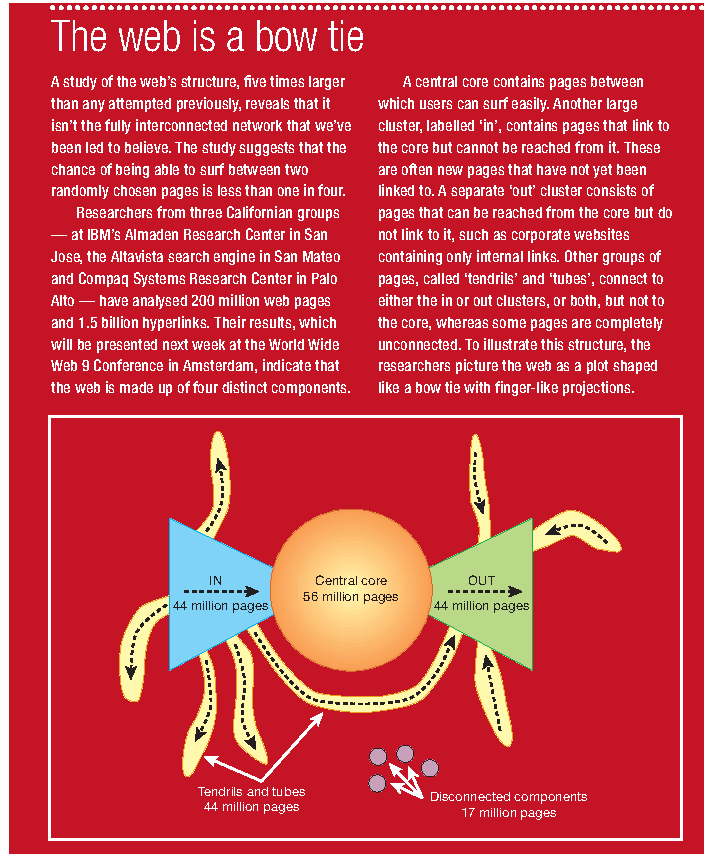
\includegraphics[width=1.\textwidth]{figs/pdf/BowTieExtract}%{WebBowTie}

    \column{0.4\textwidth}
    \href{http://www.nature.com/nature/journal/v405/n6783/pdf/405113a0.pdf}{\tiny \copyright \underline{\textit{Nature}} 405, 113 (11 May \underline{2000})}

    \begin{block}{Web as ``bowtie''}
      \begin{itemize}
      \item in-component
      \item out-component
      \item tendrils
        \begin{itemize}
        \item tubes
        \item isolated components
        \end{itemize}
      \end{itemize}
    \end{block}

    \pause
%     Three questions naturally come to mind:
%     Does the sequence I k always converge?
%     Is the vector to which it converges independent of the initial vector I 0?
%     Do the importance rankings contain the information that we want? 
% - See more at: http://www.ams.org/samplings/feature-column/fcarc-pagerank#sthash.lzdlgcBE.dpuf
    \begin{block}{\alert{Problems}}
      \begin{itemize}
      \item \structure{dead-ends} %: no links out
      \item \structure{spider traps} %: have outlinks, but never link to any other pages
      \end{itemize}
    \end{block}
  \end{columns}
\end{frame}
%%%%%%%%%%%%%%%%%%%%%%%%%%%%%%%%%%%%%%%%
\begin{frame}{\PageRank : The model}{Avoiding dead ends by dropping}
  % A matrix whose column sums are at most 1 is called \structure{substochastic}
  \begin{columns}
    \column{0.45\textwidth}
    \includegraphics<1>[width=1.\textwidth]{figs/tex/graph_dead_end}
    \includegraphics<2>[width=1.\textwidth]{figs/tex/graph_dead_end1}
    \includegraphics<3>[width=1.\textwidth]{figs/tex/graph_dead_end2}
    \includegraphics<4>[width=1.\textwidth]{figs/tex/graph_dead_end3}

    \column{0.55\textwidth}
    \begin{exampleblock}{Handling dead ends}% by dropping
      \footnotesize
      \begin{itemize}
      \item<1> ${\Pr} = \left[\begin{matrix}\frac{1}{5}&\frac{1}{5}&\frac{1}{5}&\frac{1}{5}&\frac{1}{5}\end{matrix}\right]^T$
      \item<2> ${\Pr} = \left[\begin{matrix}\frac{1}{4}&*&\frac{1}{4}&\frac{1}{4}&\frac{1}{4}\end{matrix}\right]^T$
      \item<3> ${\Pr} = \left[\begin{matrix}0.18&*&0.36&0.18&0.27\end{matrix}\right]^T$
      \item<4> ${\Pr} = \left[\begin{matrix}0.18&0.42&0.36&0.18&0.27\end{matrix}\right]^T$
    \end{itemize}
  \end{exampleblock}

  \end{columns}
    \begin{block}{Algorithm: dropping dead ends (for substochastic $M$)} 
      % A matrix whose column sums are at most 1 is called \structure{substochastic}
      \begin{enumerate}
      \item<1,2> \structure{Backward graph reduction}: remove dead ends iteratively
      \item<1,3> \structure{Compute {\PageRank}s} of reduced graph
      \item<1,4> \structure{Forward \PageRank computing}
      \end{enumerate}
    \end{block}
\end{frame}
%%%%%%%%%%%%%%%%%%%%%%%%%%%%%%%%%%%%%%%%
\begin{frame}{\PageRank : The model}{Teleporting}
  \begin{columns}
    \column{0.45\textwidth}
    \includegraphics<1>[width=1.\textwidth]{figs/tex/graph_dead_end}
    \includegraphics<2->[width=1.\textwidth]{figs/tex/graph_dead_end_pagerank}

    \begin{exampleblock}{{\PageRank}s with $\beta = 0.8$} %Classical 
      \footnotesize
      \begin{itemize}
      \item<1> ${\Pr}^0 = \left[\begin{matrix}\frac{1}{5}&\frac{1}{5}&\frac{1}{5}&\frac{1}{5}&\frac{1}{5}\end{matrix}\right]^T$
      \item<2> ${\Pr}^{\infty} = \left[\begin{matrix}0.14&0.32&0.21&0.12&0.2\end{matrix}\right]^T$
      \end{itemize}
    \end{exampleblock}

    \column{0.55\textwidth}
    \begin{block}{Idea}
      Introduce small probability $\structure{1-\beta}$ of \structure{teleporting} to a random page (usually $0 < {1-\beta}\le 0.2$)
      % \structure{
        \begin{align}
          {\Pr}' &= \beta \cdot M \cdot {\Pr} + (1-\beta) \frac{\ones}{n} \\
          {\Pr}'(x) &= \frac{1-\beta}{n} + \beta \sum_{y \to x} \frac{\Pr(y)}{\deg^+(y)}
        \end{align}
        % }
        
        \begin{itemize}\small
        \item Brin and Page: 50-100 iterations to converge
        % \item convergence depends on the $\lambda_2$
        % \item link structure of the Web $\lambda_2 \approx 0.9$
        \end{itemize}
    \end{block}
  \end{columns}
\end{frame}
%%%%%%%%%%%%%%%%%%%%%%%%%%%%%%%%%%%%%%%%
\subsection{Implementation using \MapReduce}
%%%%%%%%%%%%%%%%%%%%%%%%%%%%%%%%%%%%%%%%
\begin{frame}{\PageRank : \MapReduce}{\MapReduce workflow}
  \begin{center}
    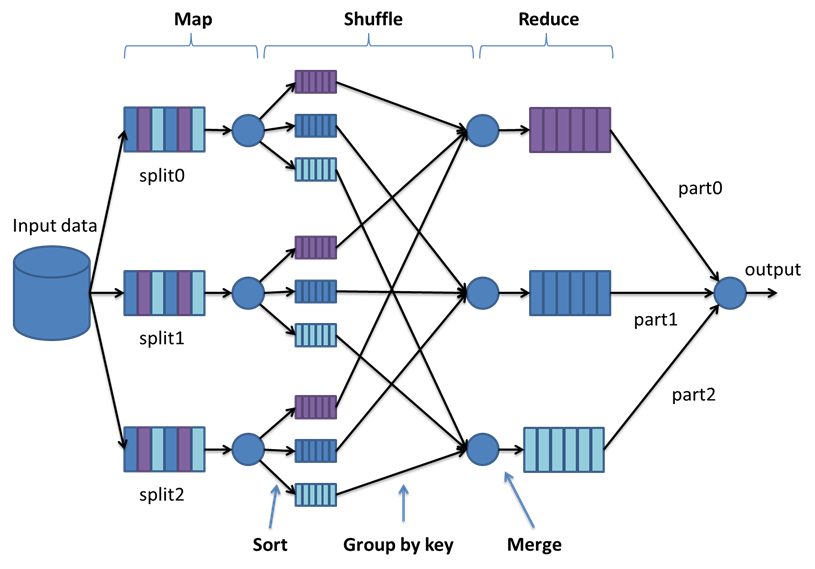
\includegraphics[width=.9\textwidth]{figs/extras/mapreduce}
  \end{center}
\end{frame}
%%%%%%%%%%%%%%%%%%%%%%%%%%%%%%%%%%%%%%%%
\begin{frame}{\PageRank : \MapReduce}{Word count with \MapReduce}
  \begin{center}
    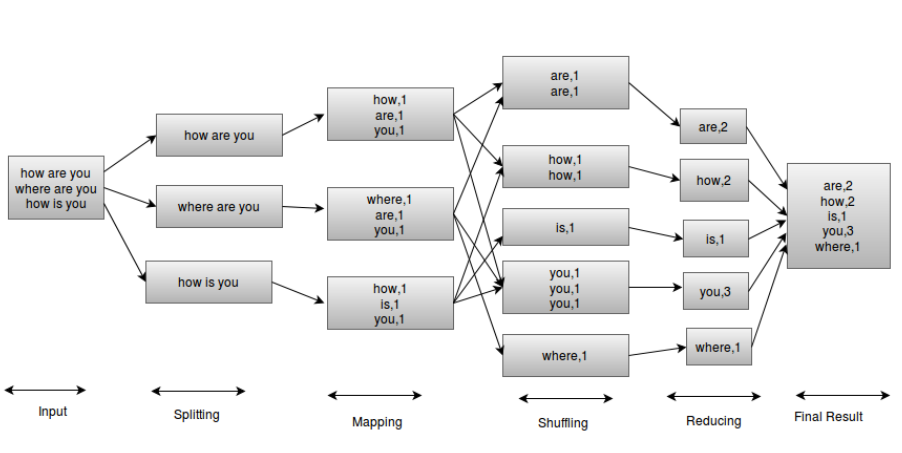
\includegraphics[width=1.0\textwidth]{figs/extras/mapreduce-wc}
  \end{center}
\end{frame}
%%%%%%%%%%%%%%%%%%%%%%%%%%%%%%%%%%%%%%%%
\begin{frame}{\PageRank : \MapReduce}{GFS}
    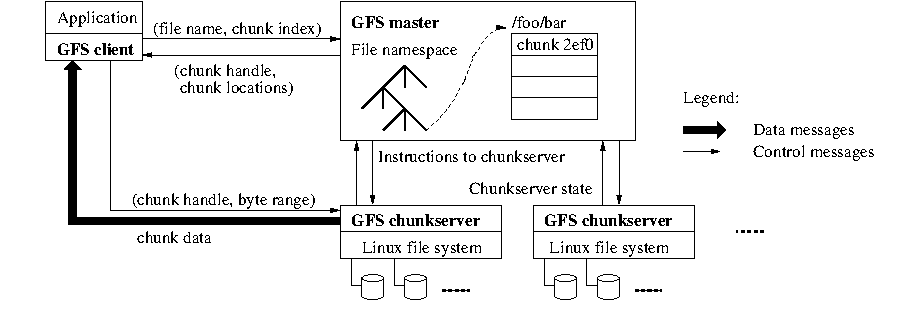
\includegraphics[width=1.12\textwidth]{figs/pdf/gfs}%{WebBowTie}

    \href{http://static.googleusercontent.com/media/research.google.com/en//archive/gfs-sosp2003.pdf}{\tiny \copyright 
      Ghemawat, S.; Gobioff, H.; Leung, S.-T. \textit{The Google File System}, Google}
\end{frame}
\begin{frame}{\PageRank : \MapReduce}{GFS}
  \begin{center}
    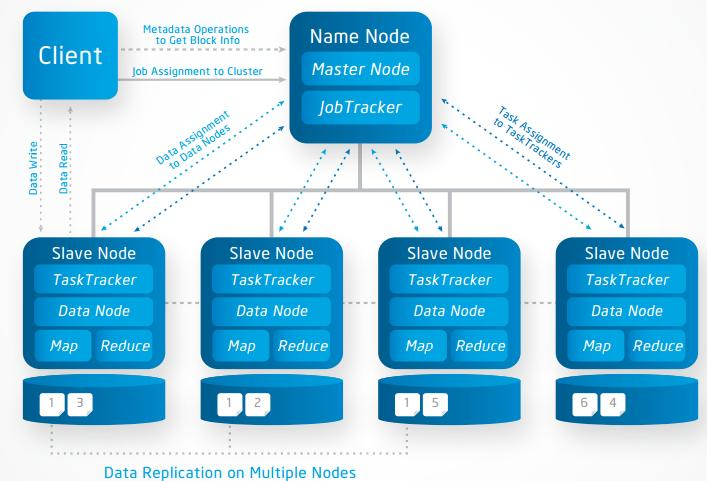
\includegraphics[width=.9\textwidth]{figs/extras/GFS2}
  \end{center}
\end{frame}
%%%%%%%%%%%%%%%%%%%%%%%%%%%%%%%%%%%%%%%%
\begin{frame}{\PageRank : \MapReduce}{\PageRank using \MapReduce}
  \begin{block}{Mapper (node $y$)}
    \begin{algorithm}[H]
      \SetKwFunction{Batched}{Batched}

      \KwData{$\braket{y}{\{x_1,...,x_k\}, \Pr(y)}$ (node -- outlinks)}
      \BlankLine

      \For{$j \in \{1,..., k \}$ }{ 
        emit $\braket{x_j}{\frac{\Pr(y)}{\deg^+(y)}}$ \;
      }
      \uncover<2>{emit $\braket{y}{\{x_1,...,x_k\}}$ \;}
    \end{algorithm}    
  \end{block}

  \begin{block}{Reducer (node $x$)}
    \begin{algorithm}[H]
      \SetKwFunction{Batched}{Batched}

      \KwData{$\braket{x}{\{ 
          \frac{\Pr(y_1)}{\deg^+(y_1)},...,\frac{\Pr(y_l)}{\deg^+(y_l)}
          \uncover<2>{,\{x_1,...,x_k\}}
          \}}$ (node -- $\Delta \Pr$)}
      \BlankLine

      ${\Pr}(x) \gets \frac{1-\beta}{n} + \beta \sum_{i = 1}^{l} \frac{\Pr(y_i)}{\deg^+(y_i)}$
    \end{algorithm}    
  \end{block}
\end{frame}
% http://toolbarqueries.google.com/tbr?client=navclient-auto&ch=[HASH]features=Rank&q=info:[URL]&num=100&filter=0
%%%%%%%%%%%%%%%%%%%%%%%%%%%%%%%%%%%%%%%%
\subsection{Modifications}
%%%%%%%%%%%%%%%%%%%%%%%%%%%%%%%%%%%%%%%%
\begin{frame}{\PageRank : Modifications}{Topic-sensitive \PageRank}
  % Haveliwala, Taher (2002). "Topic-Sensitive PageRank"
  \begin{block}{How to organize private \PageRank for each user?}
    \begin{itemize}
    \item \structure{classify users by interest} in each of the selected topics
    \item one \structure{$\Pr$ vector for each} of some small number of \structure{topic}s
    \item \structure{biase the PageRank} to favor pages of that topic
      \uncover<2>{
      \structure{
          \begin{align*}
            {\Pr}' &= \beta \cdot M \cdot {\Pr} + (1-\beta) \frac{\ones_S}{\abs{S}}
          \end{align*}
        }
        \begin{itemize}
        \item $S$ -- set of pages belonging to a certain topic (\structure{teleport set})
        \end{itemize}
      }
    \end{itemize}
  \end{block}
\end{frame}
%%%%%%%%%%%%%%%%%%%%%%%%%%%%%%%%%%%%%%%%
\begin{frame}{\PageRank : Modifications}{Link spam and \TrustRank}
  \begin{exampleblock}{}
    Yet the war between those who want to make the Web useful and those
    who would exploit it for their own purposes is never over.

    \href{http://static.googleusercontent.com/media/research.google.com/en//archive/gfs-sosp2003.pdf}{\tiny \copyright 
      Jeffrey D. Ullman %(from discussion about \PageRank)
    }
  \end{exampleblock}

  \begin{columns}
    \column{.7\textwidth}
    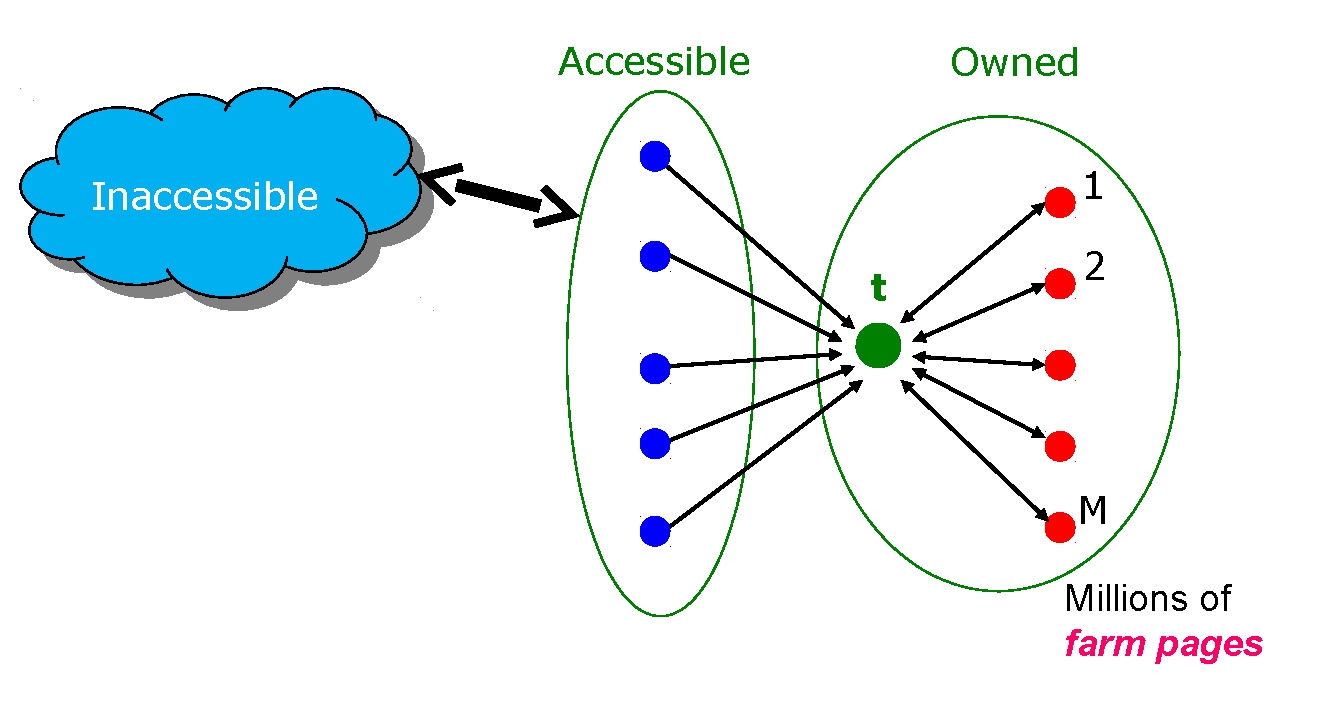
\includegraphics[width=\textwidth]{figs/pdf/spamfarm}

    \column{.4\textwidth}
    \begin{itemize}
    \item $n$ pages in total
    \item $m$ supporting pages
    \item 1 target page $t$
    \end{itemize}
  \end{columns}
  \begin{equation*}
    \Pr(t) = \Pr(\text{access.}) + \beta m 
    \underbrace{\left( \frac{\beta \Pr(t)}{m} + \frac{1-\beta}{n} \right)}_{\Pr(\text{supporting page})}
    \approx
    \structure{\frac{\Pr(\text{access.})}{1-\beta^2}} + \frac{\beta}{1+\beta} \frac{m}{n}
  \end{equation*}
  % http://www2007.org/workshops/paper_102.pdf
\end{frame}
%%%%%%%%%%%%%%%%%%%%%%%%%%%%%%%%%%%%%%%%
\begin{frame}{\PageRank : Modifications}{Link spam and \TrustRank}
  % Techniques for preventing link spammers (search-engine optimization)
  % \begin{itemize}
  % \item topic-sensitive \PageRank
  % \item \TrustRank
  % \end{itemize}
  \begin{exampleblock}{\TrustRank}
    Topic-sensitive \PageRank, where the ``topic'' is a set of pages believed to be trustworthy
    
    \begin{itemize}
    \item \structure{suitable teleport set}: 

      domain whose membership is controlled (e.g., \texttt{.edu})
      \pause
    \item \structure{spam mass}
      \begin{equation*}
        \texttt{SpamMass}(y) = \frac{\text{\PageRank}(y) - \text{\TrustRank}(y)}{\text{\PageRank}(y)}
      \end{equation*}
      negative (small positive) $\texttt{SpamMass}(y)$ $\implies$ $y$ is probably not a spam
  \end{itemize}
  \end{exampleblock}
\end{frame}
%%%%%%%%%%%%%%%%%%%%%%%%%%%%%%%%%%%%%%%%
\subsection{\PageRank as an orthogonal iteration}
%%%%%%%%%%%%%%%%%%%%%%%%%%%%%%%%%%%%%%%%
\begin{frame}{\PageRank as an orthogonal iteration}{Eigenvectors \& convergence of OI}
  \begin{definition}
  \structure{Eigenvalues} ({\small $\lambda_1 \ge \lambda_2 \ge ... \ge \lambda_n$}) 
  and \structure{eigenvectors}:% ({\small $\norm{v_i} = 1$}): 
  \begin{align*}
    \structure{A v_i} = \structure{\lambda_i v_i}
  \end{align*}
\end{definition}

\begin{block}{Convergence of orthogonal iteration}
  \small
  Let $\lambda_i \neq \lambda_j$, $v_i^*\cdot v_j = 0$, $\norm{v_i} = 1$. 

  Take arbitrary $u = c_{1}v_{1} + c_{2}v_{2} + \cdots + c_{n}v_{n}$
  \begin{align*}
    A^{k}u & =  c_{1}A^{k}v_{1} + c_{2}A^{k}v_{2} + \cdots + c_{n}A^{k}v_{n} \\ 
           & =  c_{1}\lambda_{1}^{k}v_{1} + c_{2}\lambda_{2}^{k}v_{2} + \cdots + c_{n}\lambda_{n}^{k}v_{n} \\ 
           & =  c_{1}\lambda_{1}^{k} \left( v_{1} + \frac{c_{2}}{c_{1}}\left(\frac{\lambda_{2}}{\lambda_{1}}\right)^{k}v_{2} + \cdots + \frac{c_{n}}{c_{1}}\left(\frac{\lambda_{n}}{\lambda_{1}}\right)^{k}v_{n}\right)
    \\
    \structure{v_1} &\structure{\approx \frac{1}{c_{1}\lambda_{1}^{k}} A^{k}u + {\cal O}\left(\frac{\lambda_{2}}{\lambda_{1}}\right)^{k}}
  \end{align*}
\end{block}
\end{frame}
%%%%%%%%%%%%%%%%%%%%%%%%%%%%%%%%%%%%%%%%
\begin{frame}{\PageRank as an orthogonal iteration}{Convergence of \PageRank}
  \begin{columns}
    \column{.5\textwidth}
    \structure{\fbox{Find $v_i$: $A v_i = \lambda_i v_i$}}
    \begin{block}{Orthogonal iterations}
      \begin{algorithm}[H]
        \KwData{$A$, $k$}
        \KwResult{$Q$}
        \BlankLine

        Choose initial guess for $Q$ {\small (random orthonormal $n \times k$ matrix)} \;

        \While{$\text{error}{(Q)} > \epsilon$ }{
          $V \gets A Q$ \;
          $Q \gets \text{Orthonormalize}(V)$
        }
      \end{algorithm}
    \end{block}
    \column{.5\textwidth}
    \structure{\fbox{Find $\Pr$: $M \cdot \Pr = 1 \cdot \Pr$}}
    \begin{block}{\PageRank iterations}
      \begin{algorithm}[H]
        \KwData{$M$, $1$}
        \KwResult{$\Pr$}
        \BlankLine

        Choose initial guess for $\Pr$ {\small ($\Pr = \ones/n$)} \;

        \While{$\text{error}{(\Pr)} > \epsilon$ }{
          $\Pr \gets M \cdot \Pr$ \;
          \sout{$\text{Orthonormalize}(\Pr)$}
        }
      \end{algorithm}
    \end{block}
  \end{columns}

\begin{itemize}\small
\item convergence depends on the $\lambda_2$
\item link structure of the Web $\lambda_2 \approx 0.9$
  \begin{align*}
    M = 
  \end{align*}
\end{itemize}

\end{frame}
%%%%%%%%%%%%%%%%%%%%%%%%%%%%%%%%%%%%%%%%
\begin{frame}{\PageRank as an orthogonal iteration}{Structured orthogonal factorization}
  \begin{columns}
    \column{.5\textwidth}
  \begin{block}{Orthogonal iterations}
    \begin{algorithm}[H]
      \KwData{$A$, $k$}
      \KwResult{$Q$}
      \BlankLine

      Choose initial guess for $Q$ {\small (random orthonormal $n \times k$ matrix)} \;

      \While{$\text{error}{(Q)} > \epsilon$ }{
        $V \gets A Q$ \;
        $Q \gets \text{Orthonormalize}(V)$
      }
    \end{algorithm}
  \end{block}
    \column{.5\textwidth}
  \begin{block}{\PageRank iterations}
    \begin{algorithm}[H]
      \KwData{$M$, $1$}
      \KwResult{$\Pr$}
      \BlankLine

      Choose initial guess for $\Pr$ {\small ($\Pr = \ones/n$)} \;

      \While{$\text{error}{(\Pr)} > \epsilon$ }{
        $\Pr \gets M \cdot \Pr$ \;
        \sout{$\text{Orthonormalize}(\Pr)$}
      }
    \end{algorithm}
  \end{block}
\end{columns}
\end{frame}

\section{Decentralized OI}

%Kempe-McSherry
\subsection{Serial BSOI algorithm}


\begin{frame}{Basic algorithms}{Complexity}  
  \begin{block}{Operation counts}
    \begin{center}
      \rowcolors[]{1}{blue!20}{blue!10} %\rowcolors{1}{Blue!20}{Blue!5}
      \begin{tabular}{r|l|c|c|c}
        \toprule
        Phase & Routine & Additions & Multiplications & Total Flops  \\
        \hline
        I&{\tt BSOF} & 
        $\displaystyle\Theta\left(\frac{23}{3} n^{3} p\right)$
        & $\displaystyle\Theta\left(\frac{23}{3} n^{3} p\right)$
        & $\displaystyle\Theta\left(\frac{46}{3} n^{3} p\right)$\\
        II&{\tt BSTRI\_RV} & 
        $\displaystyle\Theta\left(\frac{1}{2} n^3 p^{2}\right)$
        & $\displaystyle\Theta\left(\frac{1}{2} n^3 p^{2}\right)$
        & $\displaystyle\Theta\left(n^3 p^{2}\right)$\\
        \cline{2-5}
        &{\tt BSTRI\_CV} & 
        $\displaystyle\Theta\left(n^3 p^{2}\right)$
        & $\displaystyle\Theta \left(n^3 p^{2}\right)$
        & $\displaystyle\Theta \left(2 n^3 p^{2}\right)$\\
        III&{\tt BSOI} & 
        $\displaystyle\Theta \left(3 n^3 p^2\right)$
        & $\displaystyle\Theta \left(3 n^3 p^2\right)$
        & $\displaystyle\Theta \left(6 n^3 p^2\right)$\\
        \bottomrule  
      \end{tabular}
    \end{center}
    \pause
    To sum up, 
    \[
    \fbox{
      $\text{Total complexity} = \alert{\displaystyle\Theta\left(\frac{7}{2} n  N^2\right)}$}
    \]
  \end{block}
\end{frame}


\section{Experimental results and analysis}

\begin{frame}{Experimental results}{Experimental setup}
  \renewcommand*\DTstyle{\sffamily\small}
  \renewcommand*\DTstylecomment{\footnotesize\textsl}
  \DTsetlength{0.2em}{1em}{0.2em}{0.4pt}{0.4pt}
  \begin{itemize}
  \item \structure{Hardware}
    \begin{columns}
      \begin{column}{.5\textwidth}
        \dirtree{%
          .1 \structure{Single-GPU}\DTcomment{Hybrid node at UCD}.
          .2 2 $\times$ Intel Xeon X5670.
          .3 6-cores, 2.9GHz.
          .2 1 $\times$ %% CUDA-enabled
          NVIDIA GTX480. %, Fermi
          .3 15 SMs $\times$ 32 cores.
        }
      \end{column}
      \begin{column}{.5\textwidth}
        \dirtree{%
          .1 \structure{Multi-GPU}\DTcomment{Dirac cluster at NERSC}.
          .2 2 $\times$ Intel Xeon E5530. %Nehalem
          .3 4-cores, 2.4 GHz.
          .2 4 $\times$ NVIDIA Tesla C1060.
          .3 240 cores. %1.296 GHz
        }
      \end{column}
    \end{columns}

  \item \structure{Software}
    \begin{itemize}
    \item POSIX threads for threading in step 2 of \Bsoftri
    \item CuBlas, Magma, and Intel's MKL for LAPACK interface
    \end{itemize}
    
  \item \structure{Codes}
    \begin{itemize}
    \item stand-alone CPU, stand-alone GPU, and hybrid CPU+GPU implementations
    \item publicly available at
      \url{https://github.com/SGo-Go/BSOFI}
    \end{itemize}
  \end{itemize}
\end{frame}

%% \frame[plain]{\centering
%%   \Huge Thank you for your attantion!
%%   \includegraphics[height=0.5\textheight]{figs/extras/question.jpg}
%% }
\end{document}
